\documentclass[whitelogo]{tudelft-report}
    \usepackage{natbib}
    \usepackage{changes}
    \begin{document}
    
    %% Use Roman numerals for the page numbers of the title pages and table of
    %% contents.
    \frontmatter
    
    %% Uncomment following 19 lines for a cover with a picture on the lower half only
    %\title[tudelft-white]{Title}
    %\subtitle[tudelft-cyan]{Optional subtitle}
    %\author[tudelft-white]{J.\ Random Author}
    %\affiliation{Technische Universiteit Delft}
    %\coverimage{cover.jpg}
    %\titleoffsetx{10cm}
    %\titleoffsety{10cm}
    %\afiloffsetx{1cm}
    %\afiloffsety{18cm}
    %\covertext[tudelft-white]{
    %    \textbf{Cover Text} \\
    %    possibly \\
    %    spanning 
    %    multiple 
    %    lines
    %    \vfill
    %    ISBN 000-00-0000-000-0
    %}
    %\makecover
    
    %% Uncomment following 16 lines for a cover with a picture on the lower half only
    \title[tudelft-white]{Towards global consensus on trust}
    \subtitle[tudelft-black]{Aggregation of temporal PageRank trust vectors}
    \author[tudelft-white]{J.\ Harms}
    \affiliation{Technische Universiteit Delft}
    \coverimage{cover.jpg}
    \setpagecolor{tudelft-cyan}
    % \makecover[split]
    
    
    %% Include an optional title page.
    % \begin{titlepage}


\begin{center}

%% Insert the TU Delft logo at the bottom of the page.

%% Print the title in cyan.
{\makeatletter
\largetitlestyle\fontsize{64}{94}\selectfont\@title
%\largetitlestyle\color{tudelft-cyan}\Huge\@title
\makeatother}

%% Print the optional subtitle in black.
{\makeatletter
\ifx\@subtitle\undefined\else
    \bigskip
   {\tudsffamily\fontsize{22}{32}\selectfont\@subtitle}    
    %\titlefont\titleshape\LARGE\@subtitle
\fi
\makeatother}

\bigskip
\bigskip

by
%door

\bigskip
\bigskip

%% Print the name of the author.
{\makeatletter
%\largetitlefont\Large\bfseries\@author
\largetitlestyle\fontsize{26}{26}\selectfont\@author
\makeatother}

\bigskip
\bigskip

to obtain the degree of Master of Science
%ter verkrijging van de graad van Master of Science

at the Delft University of Technology,
%aan de Technische Universiteit Delft,

to be defended publicly on Tuesday January 1, 2013 at 10:00 AM.
%in het openbaar de verdedigen op dinsdag 1 januari om 10:00 uur.

\vfill

\begin{tabular}{lll}
    Student number: & 1234567 \\
    Project duration: & \multicolumn{2}{l}{March 1, 2012 -- January 1, 2013} \\
    Thesis committee: & Prof.\ dr.\ ir.\ J.\ Doe, & TU Delft, supervisor \\
        & Dr.\ E.\ L.\ Brown, & TU Delft \\
        & Ir.\ A.\ Aaronson, & Acme Corporation
\end{tabular}
%% Only include the following lines if confidentiality is applicable.

\bigskip
\bigskip
\emph{This thesis is confidential and cannot be made public until December 31, 2013.}
%\emph{Op dit verslag is geheimhouding van toepassing tot en met 31 december 2013.}

\bigskip
\bigskip
An electronic version of this thesis is available at \url{http://repository.tudelft.nl/}.
%\\[1cm]

%\centering{
\includegraphics{cover/logo_black}}


\end{center}

\begin{tikzpicture}[remember picture, overlay]
    \node at (current page.south)[anchor=south,inner sep=0pt]{
        
\includegraphics{cover/logo_black}
    };
\end{tikzpicture}

\end{titlepage}


    
    % \chapter*{Preface}
\setheader{Preface}

The big hype around Bitcoin and other cryptocurrencies seems to create a distorted picture of the 
original idea of a distributed, democratic financial system. The general public does not appreciate
the simplicity and brilliance of the concept but rather the price swings and the
possibility to become rich. 

A similar distortion happened to the internet itself. Once envisioned as an 
open and free network for information exchange, the World Wide Web has been transformed into an
infrastructure for commerce, data collection and cyber attacks. Certainly, many companies have created 
solutions that simplify our lives significantly. But the free use of all kinds of services comes at 
an invisible cost. Slowly, that cost becomes more visible as targeted misinformation campaigns are
dismantling democracies and data collection policies of the big internet monopolies are uncovered.

Decentralization is a natural solution to this problem. Some fundamental services such as transferring
money, communication and the access to information should not be controlled by single entities and 
exploited for profit. In the same sense, creating trust with other internet users should be 
enabled through a decentralized system. This is the motivation to contribute to the design of a
distributed trust system.

Working on this thesis has been a journey through many fields of science, from evolution theory and 
social sciences to synchronization methods of replicated databases. 
It has in many ways opened my eyes to the problems of centralized 
organizations and the advantages that distributed systems offer. Also, it sparked my interest in 
trust, cooperation and their relation to problems of society.

I would like to thank my supervisor Dr.\ Johan Pouwelse for his enthusiasm, infinitely large pool of
ideas and suggestions as well as his invaluable feedback. I thank the Tribler team for keeping me 
awake with coffee and the review work of Quinten and Martijn. I thank my parents, my girlfriend, Lyla, 
and my closest friends for their support in moments of self-doubt. A special thanks goes to my 
housemates Marnix and Liesette who helped me through the last weeks. I would also like to thank 
Alexander for our interesting talks at lunch. Without you it wouldn't have been possible.


\begin{flushright}
{\makeatletter\itshape
    \@author \\
    Delft, August 2018
\makeatother}
\end{flushright}


    
    % \tableofcontents
    
    %% Use Arabic numerals for the page numbers of the chapters.
    \mainmatter
    
    \chapter{Introduction}
\label{chap:introduction}
% \subtitle{Building a distributed reputation system as the basic infrastructure for creating trust 
% between relative strangers for the future digital economy.}

% \paragraph{Abstract.} Trust enables cooperation which in the long-term increases welfare for all 
% parties, but centralization creates an unhealthy information and, thus, power asymmetry. The future 
% digital economy will be driven by global cooperation between relative strangers; that cooperation 
% will be facilitated by distributed reputation systems without central ownership or control. This 
% work extends the scalable TrustChain fabric with an explicit, unambiguous, public representation of 
% the entities' states, thereby making sharing of information incentive-compatbile and putting another
% pillar for the trustful internet in place.

% 1. Since the ground-breaking work of Darwin we know that evolution of species is guided by natural selection, so mutation and inheritance lead to the strongest variation surviving. However, the classic view of the strongest survives does not explain how cooperation can occur, which requires some sort of altruism. Game theory explains …
%  Nowak, Axelrod, 

Trust is the bedrock of society. From the evolution of species, global markets all the way to the 
modern sharing economy, trust has always had an important impact on almost every aspect of our lives.
Trust is built on a good reputation which in turn is created through positive outcomes of past 
interactions. The value of a good reputation also depends on how widely known that reputation is.
In small communities, knowledge about each other is gained through gossiping or personal experience. 
But local communities become less important as global communities and marketplaces become more common
through internet based applications. Still, or even more so, those internet communities depend on 
trust. Protecting and distributing the knowledge about interactions in the digital world is a tough
challenge we are faced with when designing a global trust system.

The current state-of-the-art trust building systems are online platforms for the sharing economy.
The reputation systems of Uber\footnote{https://uber.com} and AirBnB\footnote{https://airbnb.com} are
an essential part of their business. The good reputation allows commuters to trust their driver and
get into the car of a stranger, or allows house owners to rent their home to a couple from the other
side of the world. The reputation of drivers and renters are stored on the platforms, they are both
valuable to the people as well as the company. This leads to problems when renters do not agree with
updates to the platform: they cannot take their reputation and move to a competitor. Users are locked
into those platform, giving platforms great power and influence. 

A similar situation exists in the banking world. Banks are entrusted with their clients money, but 
their power led to corruption and the trust was abused. The situation escalated in the 2007-08 
financial crisis which led to a global recession. The crisis inspired a new solution: Bitcoin. Bitcoin
is supposed to enable secure payments without banks. As such it removes power from financial 
institutions and puts it back into the hands of the actual owners of the money. 

Not every digital money transaction should require a bank, and similarly not every trustful
interaction on the internet should require a third-party. Instead, the ability to prove one's trustworthiness
on the internet should be open and free for anyone. Our vision is therefore to create a universal
mechanism to create trust. This work sets an important 
step towards creating such a system. Specifically we propose a mechanism that protects and 
distributes the records of transaction which are essential for creating trust. 

This first chapter introduces some key concepts around trust and explains the context of this work.
It should shed light on the origin of trust research and its significance for the future of the 
internet. A thorough contextual basis is created for the reader to fathom the problem description
and proposed solution in the following chapters.

\section{Trust research}
Virtually everyone that is part of a social community understands the concept of trust, yet defining
trust scientifically is hard. This is also due to the fact that trust is studied in a diverse set 
of sciences: evolutionary biology, sociology, economics and lately computer science. In the simplified
form of a model trust can well be described and studied. The prisoner's 
dilemma\cite{chammah1965prisoner} is one such model from game theory that creates a framework for 
understanding trust. It is widely used in research and is the basis for many experimental studies.
We describe in the following the game, it's relation with cooperation and the impact on evolutionary
theory, economics and computer networks.

\subsection{Prisoner's dilemma}
\label{sec:prisoner}
The game Prisoner's dilemma describes a dilemma common in many real-world situations, for
example the problem of two partners caught for a crime that are questioned in two separate rooms. 
Each prisoner has two options, either deny all allegations, which is more generally called cooperating
 or betray the partner, which is called defecting in general game theory. If both stay 
silent, both will get a sentence of one year. If one betrays the other, the snitch is set free while the 
betrayed gets three years in prison. If both betray each other, they both have to serve two years.
When analyzing the game without any additional knowledge and considering the payoffs for one of the
prisoner's it is always advantageous to betray the other. Either the other also betrays, in which case
two years is better than three, or the other stays silent in which case betraying sets us free. 
However, when considering both prisoners' outcomes together it would be best for both to stay silent.


While the game is quite simple the implications are far reaching. The game is able to show the 
connection between trust and cooperation. If both prisoners trust each other to never betray a 
partner, both will cooperate and get a small sentence, the best combined outcome. Yet any mistrust
makes both fail at beating the system. The problem also describes many real world problems, called 
the tragedy of the commons. For example, the global warming is a problem that can only be solved if
all peoples and all nations cooperate. Yet, the low cost and convenient usability of fossil fuels 
make it advantageous to defect and damage the environment. Either the others try to save the environment
in which case a single defection will have a small impact, or the other will also damage the environment
in which case a single cooperator will fail anyways. Only, if everyone trusts each other that
everyone does the best they can to save the environment, then it is possible to beat the tragedy 
of the commons.

\subsection{Evolution and cooperation}
\label{sec:evolution}
While cooperating, according to theory, is not necessarily a winning strategy, it is in our nature 
to do so, as has been shown by evolution theorists. The theory about competitive natural selection 
between individuals and mutation and inheritance of genes was the accepted truth about evolution 
since Darwin until in the late 1960s doubts arose about the completeness of this 
theory. When looking at group behavior in species one will find that cooperation is a common theme
among related individuals, yet there is no place for cooperation in the classic Darwin 
theory~\cite{Axelrod1390}. In their work Axelrod and Hamilton \cite{Axelrod1390} 
analyze how to combine the seemingly inferior individual's strategy of cooperating with the goal to 
maximize fitness. At the basis of their experiments is a again the Prisoner's 
Dilemma. Axelrod and Hamilton ran experiments on this game with multiple rounds instead of only one with
different strategies. They found that if the game is played repeatedly with the possibility of 
meeting the same partner again in the future, cooperation between players can be established and be
superior. Later research showed that this direct form of reciprocity, the act of returning a deed,
is only one form of cooperation found in human behavior. Nowak and 
Martin~\cite{nowak2006five} defined in total five forms in which cooperation can occur: kin selection, direct
reciprocity, indirect reciprocity, network reciprocity and group reciprocity. Conceptually these 
forms can be described like this:

\begin{itemize}
    \item kin selection: we help those that share our genes
    \item direct reciprocity: I help you, you help me
    \item indirect reciprocity: I help you, somebody helps me
    \item network reciprocity: neighbors help each other
    \item group selection: A group, in which members help each other, survives
\end{itemize}

Each concept entails at its basis trust. We trust our family, our group, our countrymen, those with whom we had a lot
of shared experiences and those we heard good things about. 
% 2. Trust in economy and digital markets …. Advance of sharing economy, ….. When talking about trust, indirect reciprocity is the method of creating cooperation. Mui created a first mathematical model which relates reputation, trust and reciprocity. According to that model reputation stems from the history of encounters 
% Mui, Martin

\subsection{Economics}
{\color{red} Old: needs to be improved}
Trust also plays a major role in our economic system and has been for the the evolution of economy 
as shown in Figure \ref{fig:economy}. In the pre-industrial age, most economy and trade was done in local
communities with families that trusted each other over generations and traders that returned year
after year. During industrial and post-industrial age companies have largely replaced local 
producers and are trusted by millions of customers based on their brand name. Nowadays, in the 
information age, internet companies allow people to connect, trade and cooperate directly, examples
being eBay for trading physical goods, AirBnb for sharing houses and Uber for ride-hailing. How trust
and the lack of it influence trade and markets has been studied in the well-known paper by 
Akerlof~\cite{akerlof1970lemons}. He describes the information asymmetry between seller, who knows
the quality of the goods which will be sold, and the buyer, who can only estimate that quality by 
some market statistic. The seller's incentive to sell goods of lesser quality than the average 
statistic leads to a decreasing statistic and thus price which in turn decreases the quality of the 
goods sellers are willing to offer for that lower price. Hence the market breaks down. Akerlof
describes institutions to solve this problem namely institutions such as guarantees, brand names and
certifications. These are trust inducing institutions and can be generalized as reputation systems.
If the sellers sell goods to many people and those people report or gossip the good quality of what
they have bought, others can trust those sellers and both seller and buyers will thrive. On the 
other hand a bad reputation will lead to a seller getting out of business as buyers will mistrust.
This closes the gap to the work of Nowak as this reputation is what makes indirect reciprocity
possible: the seller is not taking advantage of the buyer's inconvenient situation but the buyer
cannot directly return that favor. Only by gossipping the event to other potential buyers who are 
then more willingly to buy from the seller is the reciprocity circle closed.~\cite{nowak2006five}

\begin{figure}[t]
    \centering
    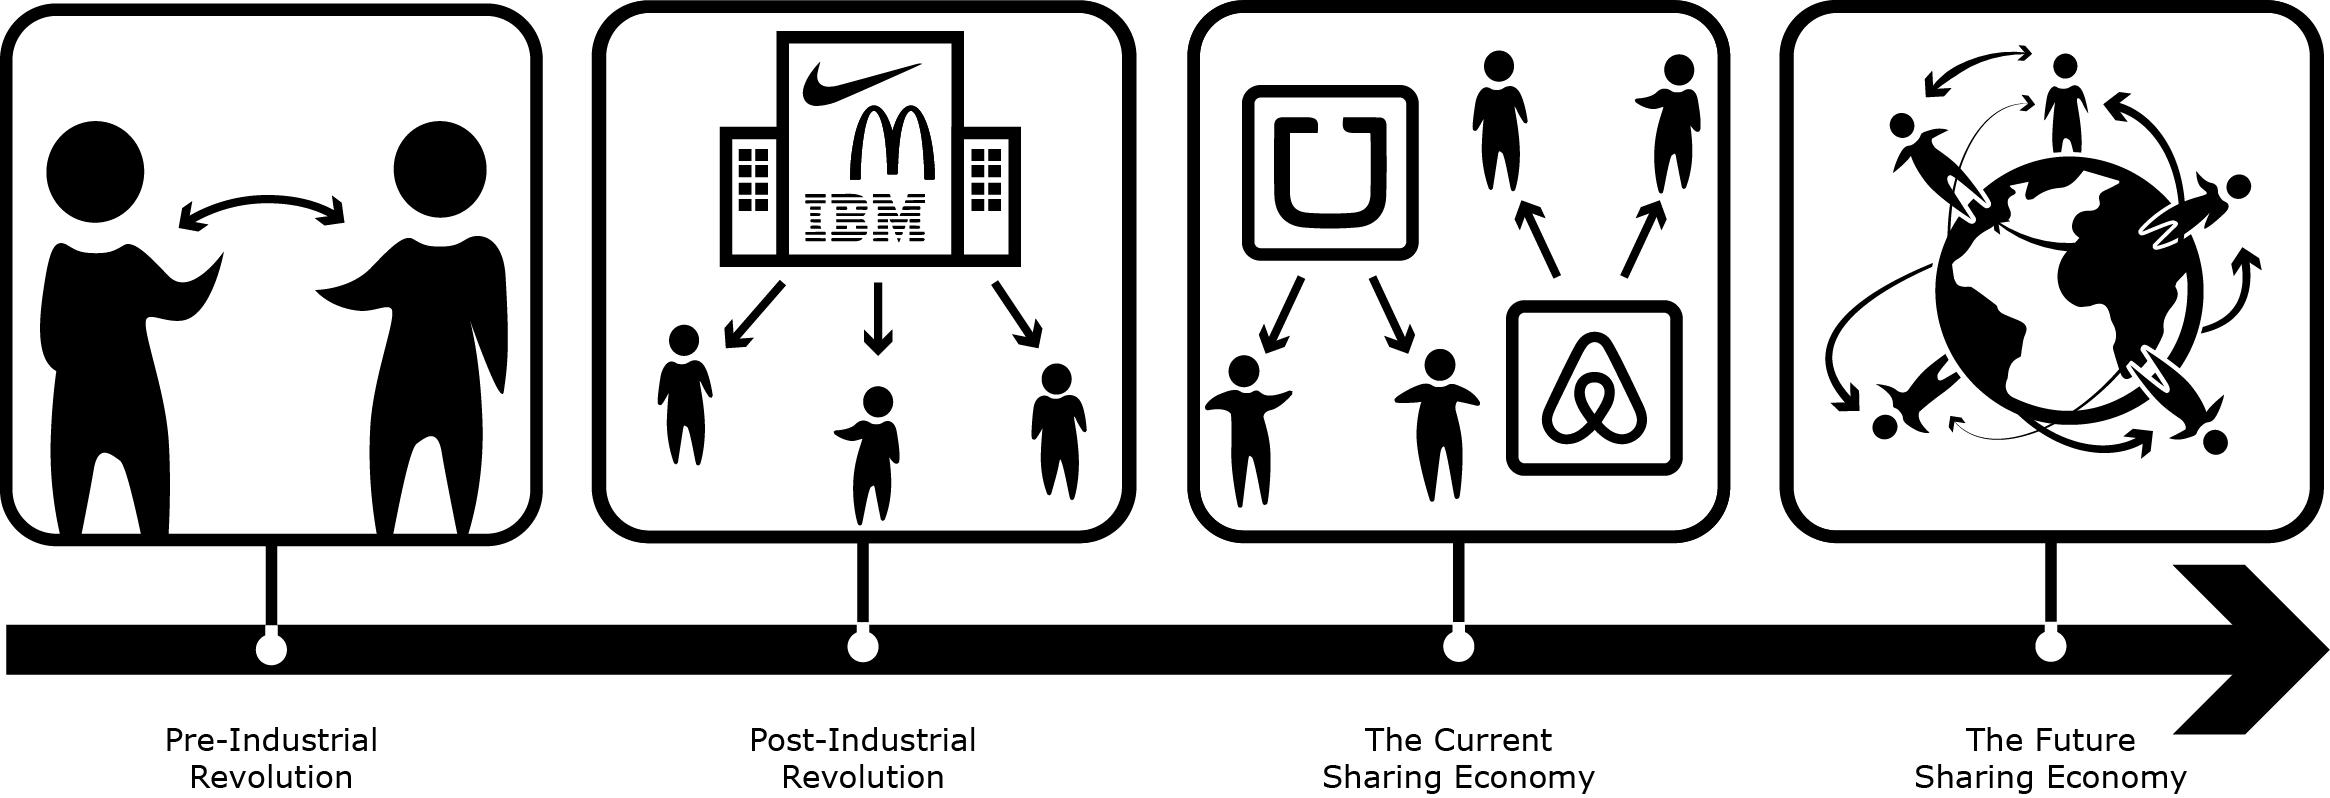
\includegraphics[width=0.8\textwidth]{images/economy.png}
    \caption{Evolution of the economy}
    \label{fig:economy}
\end{figure}

% 3. Reputation systems guide buyers towards to most trustworthy sellers on markets or help guests find houses on Airbnb that actually hold the promises made in the description. Reputation systems require three properties: dissemination, strong identities and  Yet companies take advantage of our trust and misuse our data, influence us and do not take appropriate measures to protect our data from attacks. Centralized systems are broken.
% (eBay) Ba and Pavlou, survey of reputation systems, definition of reputation system, Pouwelse 
\section{Digital trust}
{\color{red} Old: needs to be improved}
These analog, gossip-based reputation systems are what guide our decisions in buying cars, new or 
used, at which bank we store our money and at which restaurant we should have dinner.
But reputation systems are also prevalent in the digital world: we make our decisions in buying used goods 
on eBay, renting a house to a stranger (or from a stranger), getting into a stranger's car 
(what mum told us not to) based on the reputation of the partner. The sharing economy or collaborative consumption is the 
rising star of economic concepts in the information age and it is power by reputation. A company 
offers a platform on which the two sides of a trade or transaction can find each other. With each 
encounter both parties can rate that interaction and it becomes part of their history. With a longer
and more positive history the value of a profile increases as users see the reputation as security
for a good interaction and are willing to pay for it. However, there are reasons for concern. What
if the platform changes their rules in an almost unacceptable way or abuses the personal data their
users have entrusted them with? Users cannot take their reputation and data to another platform
because their reputation is actually owned by the platform facilitating the trades. Such abuses
in which trusted companies act wrongly have been happening in many times in the past, examples being
the dieselgate~\cite{VWDiesel} and the facebook/cambridge analytica scandals.~\cite{facebook} These
scandals show that even though millions of users trust them, central institutions do not necessarily
serve their customers or clients. 

% 4. The above discussion makes clear that the future digital economy requires a distributed reputation system. But making a reputation system distributed brings many additional challenges. A distributed system has no control entity which can enforce strong evidence for identities. Also single entities in a distributed system have most commonly no full view of the network, thus are not aware of all other entities or all encounters. The field is not entriely new but distributed reputation systems have been researched especially in the context of peer-to-peer file-sharing, and mobile ad-hoc system. Donation game is the game-theoretic model for this …. Although a lot of research has been conducted in the field of distributed reputation systems, major problems like the Sybil-attack, double spending, scalability and state consistency remain largely unsolved.
% Game-theoretic modeling of reputation
\section{Universal mechanism to create trust}
{\color{red} Old: needs to be improved}
We envision a future in which collaborative consumption is possible without any intermediator. This
future requires a reputation system which is application agnostic, owned by noone and ruled by 
everyone. A distributed reputation system as a layer directly
on top of the internet. However this poses some challenges from a technical
point of view. Distributed system are intrinsically hard to control and regulate, which is both 
blessing and curse. No party can impose unfair rules on other users but it is also hard to prevent 
malicious users from sending wrong information across the network. \cite{HENDRIKX2015184} reviews
state-of-the-art reputation systems and finds that all commercial reputation systems are centralized.
Some of the scientific reputation systems are decentralized like EigenTrust 
\cite{kamvar2003eigentrust}, P-Grid \cite{aberer2003p} and RateWeb \cite{malik2009rateweb}, yet
they have not been proven to work in settings where high throughput, global scaling are required 
which is the case for a global reputation system. Distributed, secure and globally scalable systems
remain an unsolved problem.

% 5. This master thesis was written in the context of the blockchain lab at TU Delft which has a long history of research on the topic of distributed reputation systems. The research is targeted at Tribler, a secure BitTorrent client which is aimed at protecting against free-riders.
% BarterCast

\section{TU Delft Blockchain Lab research}
The ambition of creating the first global trust system is realized at the Blockchain Lab of TU Delft,
which is the research group in which this thesis was created. The lab has a strong focus on exploring
new concepts, implementing them and testing them in production grade software. 

The research group has great experience and a solid track record in the field of distributed work 
systems. Especially peer-to-peer file sharing system have been studied, first and foremost the 
internally developed Tribler\footnote{https://tribler.org} application. Tribler is a client for the
BitTorrent protocol. It offers many improvements over conventional BitTorrent clients like improved
privacy and security, streaming and reputation management. It has been the testbed for algorithms of
bachelor, master and Phd students for ten years with 1 million downloads in that period. In those 
years of research several milestones have been reached. In \cite{meulpolder2009bartercast} we have 
solved the free-riding problem in the peer-to-peer file-sharing context with a reputation system 
that tracks uploads and downloads. With TrustChain \cite{OTTE2017} we have created our own 
blockchain fabric for bandwidth as a currency which builds on the previous work and adds 
tamper-proof recording and immutable history to the reputation system.

The problem of peer-to-peer file sharing systems maps well onto the trust domain. Users of BitTorrent
clients download from other users who upload data. Downloading data has benefit to users because 
they are interested in the content, however uploading has no obvious advantage. It is only necessary
to keep the content available for others. There is an obvious incentive problem, a tragedy of the 
commons. A free-rider can download without uploading, thereby consume resources without contributing.
The problem can be solved through a trust system. By recording the behavior of each user and making
it public a reputation can be assigned to each user which represents their resource usage. Users 
that contribute a lot increase their reputation while downloading decreases that reputation. Other 
users are able to inspect that past behavior of any potential partner and use it for their decision 
whether the partner deserves a contribution. 

The recording of file transactions and security of those records is facilitated by our blockchain
fabric TrustChain~\cite{OTTE2017}. TrustChain is a multi-chain fabric which lets each user create
an own chain. It is therefore built for horizontal scalability and unbounded throughput. By design,
TrustChain enables the creation of trust in any application context. The solution is implemented
in Tribler and has been used in production for more than a year as of 2018. The implementation 
details of TrustChain will be discussed more in Chapter~\ref{chap:model}. 

The great scalability of TrustChain comes at the cost of security. The architecture allows for 
attacks to be detected but the system can only be secured if honest users engage in that defensive 
behavior. This can only be ensured through incentives: agents should never be able to gain an 
advantage by circumventing the rules. 

\section{Contribution}
In this work we study a mechanism to ensure the proper dissemination and verification of transaction
records. In any trust system, the transaction records are the basis for the reputation of users and 
thus the trust users have in each other. With the records, also the reputations itself are spread, 
leading to more agreement of reputation and thus higher value. Also defending the reputation records
against attacks makes records more credible and dependable, opening applications for TrustChain with
higher requirements for security.

We will enlarge on the problem description in the next chapter. Afterwards the problem will be defined
formally and analyzed in the bounds of the definition. Before proposing a solution, some existing
approaches for recording and dissemination of data will be discussed in chapter. Next, we define a
solution based on the TU Delft blockchain fabric TrustChain and propose a specific mechanism of 
using such a fabric. Finally, we prove the correctness and scalability properties of the fabric in
experimental analysis, before concluding and making suggestions for further research.
    
    \chapter{Problem description}
In the introduction we make a case for the decentralization of applications that handle private
information or resources and argues that scalability is one of the main problems of the promising
blockchain technology to make such systems a reality. Trustchain is an approach that removes the 
main bottleneck that restricts the scalability of the most common blockchain fabrics, namely global
consensus. However the lack of agreement on a single accepted set of transactions has many 
implications for attack resistance and correctness guarantess of the system. This chapter 
introduces these implications and defines the problem that this work is supposed to tackle.

\section{Attacks}

\subsection{Double-spend attack}
One of the most challenging attacks that exist in distributed systems is the \textit{double-spend}
attack in which an adversary creates two conflicting transactions with two different agents without
telling each about the other, effectively using resources twice. In centralized systems this attack
is prevented by the central server which processed transactions in order and realizes that the 
resources were spent in the first version of the transaction. Bitcoin was the first decentralized
accounting system that solved this problem without a central, trusted entity. However the mining
which creates a single accepted sequence for transactions is costly in terms of time and resources.
Without global consensus Trustchain (discussed in more detail in section 3) is not able to prevent 
the double-spend attack. Instead, the double-spend attack will be recorded and therefore made 
detectable. The attacker sends two conflicting transactions to two different agents and keeps one,
but both partners write the conflicting blocks on their chains. If those two agents share their 
blocks with each other or both share their blocks with a third agent, the attack becomes detectable
because the two blocks are conflicting. The prevention of this attack therefore requires 
dissemination of transaction data across the network and constant checking for conflicting 
transactions by all agents.

\subsection{Sybil attack}
During a sybil attack an adversary takes control over many entities at the same time without making
this known to the network. The attacker can then use those entities to gain influence without any
real cost because the controlled entities can create proof of transactions without actually 
performing them.

This problem is very hard to detect because controlled entities can look like real agents to 
external observers. In centralized systems this is often prevented by requiring multiple 
authentication steps, for example scanning an identity card. Also if the creation of new agents has
some costs, the adversary needs to evaluate the possible advantage against the cost of creating
multiple agents.
In Bitcoin and other proof-of-work based cryptocurrencies the attack is avoided because the power
to create a new block is proportional to computational power, so whether the computational power
is spread over multiple agents or not does not matter to the voting power in the system.

For other decentralized systems the sybil attack continues to be a challenging problem. Many 
solutions have been proposed which analyze the topology of the network. Also an initial negative 
balance has been proposed by some. Specifically for the Trustchain two algorithms, namely NetFlow
and Temporal PageRank. Yet, while the two algorithms allow for sybil-resistant calculation of a 
metric which is related to the balance of agents. Also the accuracy of the algorithms depends on 
the amount of data that is available, making it neccessary to share data between agents in order
to better be able to estimate the probability of sybils. The sybil attack will further be discussed
in chapter 4.

\subsection{Blockwithholding attack}
In decentralized systems it can be advantageous for agents to not share some information about
their transactions that would otherwise render them in a weaker position. This is not possible
in centralized systems because users do not keep their own data which instead is stored on the
central server. Thus it is not the user's decision to share or not share information with others.

In common blockchain fabrics all information is shared with everyone and only information that is 
accepted by everyone is true. By removing the global consensus this guarantee is no longer intact.
If user's own their data, they can decide to share it or not. Agents can claim that information was
lost during transactions or that a transaction did not take place.

\subsection{Dishonest behaviour}
Some application types may require agents to act according to a specific set of rules. For example
in the Tribler application, if an agent (responder) receives two requests for contribution the 
agent should contribute to the one agent that has contributed the most in the past as that agent 
deserves to be rewarded for those past contributions. Without global consensus the agent determines
the ``goodness'' of the requesters on the basis of an unobserved information set, which is a subset
of the global network information. However the agent can also decide to not stick to the rules and
contribute to the lesser of the two requesters. Without consensus on the information set on the 
basis of which the responder decides, this dishonest behaviour cannot be detected and punished by
other agents.

\section{Research question}
From the above discussion it becomes clear that removing the global consensus from any blockchain
farbics opens the system to many forms of attacks. The missing guarantees on information makes it
hard to check the correct behaviour of other agents. This makes sharing of information and 
validation of transactions an essential building block of a blockchain system without global
consensus. Yet, the question is how to enforce dissemination of transaction records without a
trusted third party. Also which information is neccessary to distribute accross the network and how
can we make sure that validation of that information is done by all nodes. Formally we can define 
the following research question:

\begin{center}
    \textit{How can we design a scalable, decentralized accounting system that ensures the distribution,
    correctness and honest usage of transaction records?}
\end{center}

The research question entails some requirements for the system that we are trying to develop. In 
the following we will explain each of those in more detail.


\subsection{Accounting system}
\label{sec:accounting_system}
The system we are trying to build is an accounting system. An accounting system keeps track of 
transactions of a resource of value between at least two parties. Accounting systems have many 
applications; two common examples are a banking system and a reputation system. Each entity in 
the accounting system has a unique identifier and from the history of the transactions recorded 
in the system a certain balance can be assigned to each identifier. When a new transaction is issued 
the balance is increased or decreased and usually some threshold is put inplace to restrict the 
infinite spending of resources. This implies that the order of transactions is of importance. As an 
example consider an entity A with the balance of 5 a minimum threshold of 0 and two transaction 
spending 4 units and 3 units two parties B and C, respectively. Obviously, it is not possible that
both transactions are accepted. Either, A first spends 4 units on the interaction with B and cannot
afford the transaction with C or the other way around. If entity A tries to submit both transactions
at the exact same time, it is the task of the accounting system to create an order of two transactions
and restrict the expenditure beyond the balance threshold.

\subsection{Scalability}
Accounting systems can exist in many different sizes and contexts, they do not even have to be
digital for some applications. However in this work we are concerned with planet-scale accounting
which even enables micro-transactions with high frequency. Therefore scalability is one of the 
main factors. Before the ascent of internet applications such dimensions were unheard of but in
the last decade services such as Facebook, WeChat or YouTube have shown that an application can 
grow to have billions of users. Our ambition is to lay the theoretical and practical basis for 
future systems that scale to these sizes. In practice that means that the transaction throughput
of the global systems needs to grow with the amount of users and that no global limit is in place
that restricts further growth.

\subsection{Decentralization}
Ownership of all transaction data can, depending on the context, give the owner power, leverage and 
value. Furthermore, a central entity creates a target for attackers and with sufficient resources
available an adversary will in the end be able to compromise the system. We see accounting systems
as a part of the infrastructure that enables applications such as banking or reputation systems. No 
single entity should be owner of such infrastructure. That is why we are considering a decentralized
solution. In the context of an internet application a centralized model assumes that one single (central)
trusted entity has access to all information and all users know and connect to that single entity. In a 
decentralized model, we cannot assume that any other entity is trustworthy or omniscent. Instead entities
are equal and communicate with each other. All users know about their own transactions and are owner of
their data, with full control over whom to share them with. 

\subsection{Distribution}
In a perfectly decentralized system each entity only knows about their own transactions. For an 
accounting system that means that each entity needs to check for themselves that they do not exceed the
balance threshold. Yet, an entity's interest could be to spend as much as possbile, which makes the 
self-control mechanism ineffective. In the context of reputation systems, an entity's interest could be
to show their good behaviour to others. In those situations a distribution mechanism needs to be put 
inplace because in a decentralized system we can no longer assume that information is simply available from
the central entity. Perfect distribution of data would mean that each user is informed about each transaction
happening on the accounting system's network. However in practice such a situation virtually impossible to 
uphold, especially when scaling to global high-frequency microtransactions. A balance needs to be found 
between the distribution of information, the scalability of the system and the storage and processing 
capabilities of each entity.

\subsection{Correctness}
In order to ensure the correctness of data multiple aspects need to be considered. First of all data needs
to be stored in a tamper-proof manner, that is, once a transaction is accepted by all parties that transaction
should not be changeable afterwards. Also the order of transactions needs to be definite, the reason for 
this was explained in Section \ref{sec:accounting_system}. Finally, entities need to be able to validate the
correctness of the state of the system.
The distribution of data informs entities in the system about the behaviour of other agents, but without
validation of that data, missing or wrong information cannot be found. This is another aspect that is often
solved by a central entity that continuously analyzes the information received by users. In a decentralized
system the validation has to be performed by each entity. For example entity A has a balance of 2 units but
is trying to spend 3 units in a transaction to entity B. Without a central entity the only party to
prevent A from transaction is entity B. B is only able to detect the invalid transaction if A has shared all
it's transactions with B and if B uses some validation precedure before engaging in a new transaction. It is
important to realize that validation is only possible if information is distributed. 

\subsection{Honest usage}
Finally, the system should make it possible to ensure the honest behaviour of entities. To show how the 
previous two components are not enough to ensure this, we can continue with the example from the previous
section. So even if B knows that the balance of A is insufficient to commit the transaction, both could 
collude and still commit the transaction. Afterwards, there is no way of knowing whether B was acting 
wrong on purpose or whether A did not share its information correctly. 

In order to ensure correct usage of the given information it needs to be possible to distinguish good from
bad behaviour. Without a central entity that knows the truth about every entity it is not straightforward to 
know which entity is the responsible one for a wrong transaction.


\section{Limitations and assumptions}
    
    \chapter{Related work}

\section{Context}

\paragraph{To understand the relevance} of this work we need to put it into the
perspective of the context of reputation systems and their applications. 
With the wide-spread use of the internet for trade, sharing and communicating,
interactions between strangers living far apart are wide-spread. Many applications
allow for exploitation through manipulation and taking advantage of the asymmetry
of information. For example a buyer needs to pay for products before even seeing
and afer receiving the money the seller actually does not have any incentive to
deliver a product. This opens the door for exploitation. In order to solve this
problem a reputation system is put into place in ebay, which shows publicly what
other buyers said about the seller in the past. If the seller has not delivered
a product a few times, the reputation will tainted with negative reviews and 
buyers will be reluctant to interact with this seller in the future. Also, having
no reputation at all will seem suspicious and buyers will have little trust in
the seller. This influences the prices of products that this seller can ask for.

\subsection{Reputation systems}

Reputation is a concept that not only exists on internet platforms, but it is 
an important part of everyday life. Everyone has opinions about friends, colleagues,
companies, newspapers, weather forecasts and many more things. Reputation and 
trust are subjective quantities, we are influenced by gossip from our peers. If
all of our friends tell us that a certain company makes crappy laptops, we are
probably choosing for a different companies laptop.

In this work we will focus on reputation systems for internet platforms. In this
category there are two different approaches, the centralized approach and the 
decentralized approach.

\paragraph{Centralized} ...

\paragraph{Decentralized} ...

\subsection{Applications}

\paragraph{Market}
\paragraph{Sharing economy}
\paragraph{BitTorrent}
\paragraph{Tribler}

\section{TrustChain}

\subsection{Data structure}
\subsection{Accounting mechanism}
\paragraph{Definition of trust and reputation}
\subsection{Subjective graph}
\subsection{Consensus}



    \chapter{Attacks}

\section{Sybil attack}

\section{Block-withholding}

\section{Double-spend}

\section{Self-promoting}

\section{White-washing}

\section{Collusion attack}


    \chapter{Reputation consensus through anti-entropy}
\label{chap:mechanism}
% A specific implementation of the extension of TrustChain

% A policy that makes dissemination and verificaiton strategy-proof
In the first chapters of this thesis we introduced the incentive problem of information dissemination 
in distributed reputation systems. In the previous chapter we introduced an extension of the TrustChain
architecture that allows for agents in the network to obtain and verify each other's internal 
information state. But in order to achieve the goal of strategy-proof dissemination of information
a tangible mechanism is required that applies the advanced tools that the new architecture provides.
In this chapter we analyze one such mechanism which is based on the anti-entropy concept. We first
describe the mechanism conceptually, then discuss the implementation details and finally elaborate
on some intrinsic properties the mechanism could introduce in actual applications. In the next
chapter an implementation will be analyzed experimentally with small agent sets in order to prove
that properties from the theoretical analysis can be observed in practice.

\section{Conceptual description}
% The exact protocol: before each transaction we exchange all data and verify each other's chain

% What this allows us to do is: we can agree on a ranking that includes all of both agents data. 

% We give the receiver a chance to proof that he is worth

% We make sure that an agent has to obtain all data before making a transaction. 
Section~\ref{sec:strategy_proof_sharing} explained that the architecture itself does not solve the 
incentive problem. It rather provides the evidence on which an incentive mechanism can be built. 
Many different mechanism are possible, depending on the specific needs of the application context. 
This offers a lot of flexibility for system designers which is different from existing architectures
which a very static in their protocol and have pre-defined security and scalability properties.

\subsection{Design choice: security vs scalability}
Security, decentralization and scalability are three properties that are traded against each other 
in the design of a decentralized system. It can be argued that TrustChain was designed with scalability
as the highest priority while Bitcoin was designed with security as highest priority property. We
argue that the extension that allows for internal agent state transparency allows for flexibility in
the design choice of security and scalability. In this section we propose a mechanism that trades 
some of the scalaiblity of TrustChain for stronger security in order to show that a secure mechanism
is possible on top of the TrustChain architecture. 

\subsection{Concept: anti-entropy}
The mechanism is based on the concept of anti-entropy, which was described in \cite{demers1987epidemic}
for the purpose of maintaining mutual consistency between multiple replicas of a database. Updates
to the database can arrive at any single site and need to be forwarded to all other replicas. Demers
et. al. study three different mechanisms to disseminate the updates to other sites: direct mail, 
anti-entropy and rumor mongering.

In the direct mail mechanism, a database forwards the update to all other database immediately, which
seems like the most straight forward approach but is restricted by the fact that each database does
not know about all other databases. 

Anti-entropy is a process in which each database periodically chooses a partner database and both 
exchange all database contents in order to resolve any differences between the two. The process was
found to be reliable but slower than direct mail. 

The final mechanism is called Rumor Mongering. Sites consider updates ``hot rumors'' after receiving
them for the first time. While the site considers the rumor ``hot'', it choses periodically another
site and informs it about the rumor. When the site has encountered a certain amount of sites which
were already aware of the ``hot rumor'', that update is retained but site stops with actively
propagating the update. 

For the purpose of this work, we will focus on the concept of anti-entropy. Direct mail is not a
viable option because for large social networks the embedded social networks are a very small 
subset and the rest of the agents in the network would not be informed of updates. Rumor mongering 
effects are best observed in larger networks however this work is concerned with conceptual analysis
and the experimental analysis in the next section concerns small networks. Also there are more 
algorithms than these three but anti-entropy fits the architecture of TrustChain very well and is 
a good starting point for analyasis of dissemination mechanisms. The analysis of other mechanisms
will be subject of future work.

\subsection{Replicated databases vs TrustChain}
The context of the work of Demers et. al. is similar to the context that this work is concerned with
in many regards. Replicated databases are a distributed system as all instances of the database are
independent, equal entities, just like the agents in the TrustChain network. Each agent has an 
internal state which is equal to the set of transactions that agent is aware of which is equal to
the state of the database which is equal to the entries that database is aware of. Our goal is to 
propagate information on new transactions just like the goal of Demers et. al. was to propagate 
updates to the databases. 

In the context of reputation systems anti-entropy allows for two agents to align on their knowledge
of the social network, that is to obtain the same embedded social network and agree on the reputation
of all agents in that network.
Two agents, $a_i$ and $a_j$ have two different internal states, represented by the sets of encounters
$E_i$ and $E_j$. There can be some overlap between the two sets, but that is not guaranteed. Agent 
$a_i$ chooses to synchronize states with agent $a_j$. Both agents send their own set of known 
encounters and merge them. This results in a new set $E_{i,j} = E_i \bigcup E_j$. In the context 
of TrustChain this translates to the exchange of transaction blocks, such that after the exchange 
both agents have the exact same set of transaction blocks. As the reputation of peers is calculated
from the set of transactions both agents agree on a single reputation vector. If the two agents also
use the same function for trust calculation both can even agree on a single trust vecotr. The two 
agents have reached consensus on trust and reputation. 

The exchange of information will be recorded in the form of exchange blocks on the chain of both 
participating agents as explained in the previous chapter, section~\ref{sec:implementation_state_transparency}.

The consensus is only reached at one point in time and is not maintained. Once any of the two agents
conducts another anti-entropy exchange or a transaction, the other agent is not required to be 
informed or to observe the interaction. That is after the exchange both internal states can diverge
until the same two agents happen to perform another state synchronization. 

In the work of Demers et. al. database instances chose partners for anti-entropy exchanges at random
which is a valid strategy as each peers updates seem equally important. In contrast, reputation 
systems should value the information about possible future interaction partners as more important.
Therefore, our proposed mechanism requires agents to at least perform an anti-entropy exchange with
those agents that they will have an interaction next. That way, both parties of a transaction are 
required to obtain and verify each others information in order to make sure that the transaction 
will be done on top of a valid state. If any party does not agree with the state of the opposite 
party, the transaction will not take place. If any party performs a transaction eventhough the 
information clearly shows misconduct on the part of the partner, they will also be held responsible 
for not performing their validation responsibility. Without the requirement of validating transaction
partners, agents can purposefully exchange data with honest agents but perform interactions with 
dishonest agents and later claim to have had no knowledge of the dishonesty of the partners. 

\section{Implementation of anti-entropy exchanges}
In the previous section we described the anti-entropy method for information exchanges between 
agents. This section elaborates on the implementation details of the mechanism in the TrustChain 
architecture. We start with an application agnostic example of the exchange of information and the 
transaction process.. In the next section we expand on the considerations for application specific 
implementations.

We consider an agent $a_i$, who is about to conduct another interaction. What the interaction is 
about and how the partner is chosen are specific to the application context. For this example we 
assume that $a_i$ can randomly choose an agent from the network. Once $a_i$ has chosen a partner $a_j$,
$a_i$ starts the communication and is therefore the \textit{initiator} while $a_j$ is the \textit{responder}. 

The initiator starts the interaction by sending the chain and exchange history to the responder. The
chain{\color{red} Is this explained somewhere} includes the blocks that describe the transaction and 
exchange history {\color{red} Is this explained somewhere} of the initiator while the exchange 
history includes the index of blocks exchanged for each exchange block. On reception, the responder 
can verify the chain using the algorithm \ref{alg:verify_chain}. The algorithm first checks,
wether the chain is a complete sequence without missing blocks in between. If the check is positive,
the number of exchange and transaction blocks is compared, as well as the public keys of partners
such that each transaction can be paired with a succesful exchange previous to the transaction.

\begin{algorithm}
\caption{Chain }\label{alg:verify_chain}
\begin{algorithmic}[1]
\Procedure{verifyChain}{}
\EndProcedure
\end{algorithmic}
\end{algorithm}

Once that check also succeeds, the responder is able to build a block index that indexes the internal
state of an agent. The block index is a summary of the contents of the internal state and shows
which transactions of which agents are knwon to the agent. This is an optimization that allows agent
to request only specific blocks instead of the complete database of another agent. This is a lot 
faster if agents that already share a lot of data. Agent $a_j$ compares the calculated block index
with his own index and request the difference in blocks, so those that $a_i$ has but $a_j$ does not 
have from $a_i$.

The initiator receives the request and replies with the blocks that $a_j$ requires to perform the 
complete internal state validation. Should the responder, for whatever reason, wrongly require more
blocks, so also blocks that are not in $a_i$'s posession, the interaction will be canceled. 

The responder receives the missing blocks. At this point $a_j$ should be in the posession of all
of $a_i$'s blocks plus some blocks that $a_j$ has over $a_i$. Agent $a_j$ is then able to perform
the complete internal state verification according to algorithm~\ref{alg:verify_state}. A state is
valid if:

\begin{algorithm}
    \caption{Chain }\label{alg:verify_state}
    \begin{algorithmic}[1]
    \Procedure{verifyChain}{}
    \EndProcedure
    \end{algorithmic}
\end{algorithm}

\begin{itemize}
    \item the chain is valid as per algorithm~\ref{alg:verify_chain}
    \item the hashes of the blocks according the the exchange indexes match the hashes recorded on
    the chain's exchange blocks
    \item Any recorded misbehavior of other agents is reflected by those agents' public keys in the 
    ignore and block list
\end{itemize}

If the internal state of $a_i$ is determined to be valid by $a_j$, the responder shows approval by 
sending the own chain, exchange history and blocks (which can be calculted by taking the opposite
difference from before) to agent $a_i$. 

Once the initiator receives that data from the responder, the second validtion of chain and state, 
this time agent $a_j$ as subject, can be conducted. If also this checks out, the valdiation phase is 
completed and the initiator can publish an exchange block proposal, which includes the hashes of the
exchanged blocks. The responder receives that proposal and the hashes contained in the proposal block
match the hashes that $a_j$ calculates for the excahnged data, the block is signed and returned.

This concludes the anti-entropy exchange, after this the two agents perform a normal interaction.

\section{Consideration of application specific features}
choosing partners -- we now chose partners randomly but probably for many applications there are 
better strategies
application specific rules -- we could perform addiitonal verification for application context, for
example no downloading after a certain negative balance boundary

\section{Advanced implicaitons of anti-entropy}
locality -- when you need to exchange all information and storage has avlue, it is cheapter to 
interact with agents that have a largely similar information set
sybil attack -- when we can apply application specific rules and we require agents to perform checks
of all agents they interact with, we can introduce a rule that says agents cannot upload to agents
that are completely new to the network (they first have to prove themselves). This way an agent 
cannot create fake agents that all download from one agent and thus increase that agents balance 
without actual downloading happening


    \chapter{Experiments and results}
Theory shows that internal agent state transparency and the anti-entropy mechanism reward honesty
and punish any strategic manipulation. We implemented this mechanism and establish in this chapter
how it handles strategic manipulation. More specifically we emulate honest agents and multiple 
types of strategic manipulators in small scale experiments. We can observe the behavior of the 
honest agents and find that strategic manipulators are detected and isolated. We show that honest agents who
execute our mechanism are able to effectively detect malicious agents that do not share or do not verify their partners 
and ignore them for future interactions.

The rest of the chapter is structured as follows: we first give an overview of the software 
architecture. Then we explain the setup of the experiments and the types of strategic manipulation
that will be emulated. Finally we present the results of the experiments.

% In the previous chapters we have explored the problem of dissemination of information in distributed
% trust systems. We offered a solution in the form of our multichain based TrustChain architecture, extended 
% it with internal agent state transparency and designed a mechanism that prevents any free-riding on
% dissemination and validation of information on transactions. In this chapter we aim to prove the 
% properties of the mechanism and architecture by experimental analysis. We built a proof-of-concept
% software that fully implements the architecture and mechanism described in this work. It allows us 
% to run an emulation of an agent network and study the behavior of agents in the presence of strategic
% manipulators.

\section{Experiment design}
The goal of the experiments is to prove the true effectiveness of the mechanism at detecting 
manipulation attempts and isolating malicious agents. Three different types of dishonest behavior 
will be analyzed in the experiments.

\begin{itemize}
    \item \textbf{Dissemination free-rider}: An agent that performs transactions normally but does
    not respond to exchange requests or start own exchanges.
    \item \textbf{Validation free-rider}: An agent that performs exchanges and transactions normally
    but does not perform any validation
    \item \textbf{Forking}: An agent creates two conflicting transactions and forwards them to two 
    different partners without telling them about the other transaction.  
\end{itemize}

% The goal of the experimental analysis is to show that free-riding on dissemination and validation of
% transaction information is no longer possible with the extension of TrustChain proposed in 
% chapter~\ref{chap:state_transparency} and the mechanism in chapter~\ref{chap:mechanism}. This would
% be a major step towards a secure and valid distributed trust system. 

In the experiments we emulate small agent networks up to 6 agents. We assume that agents are trying to perform 
interactions with each other. The experiments are not concerned with the actual trust agents have 
in each other so we keep transaction blocks empty. Agents are acting completely autonomously 
but knows about all the other agents in the network. At a frequency of 20 per second agents go through
rounds, in each round an agent has a 1\% chance of starting an interaction. This adds up to approximately
1 transaction every 5 seconds. In addition agents respond to interaction requests from their peers 
asynchronously. At the start of the interaction a peer is selected with uniform probability. If an
interaction with the selected partner is already ongoing, the new interaction request is cancelled
without selecting a new partner. The same happens when the selected partner is a known malicious 
agent. Once the interaction is started honest agents perform according the mechanism as described in
chapter \ref{chap:mechanism}. The other types of agents each have some deviation from the expected
behavior in order to obtain an unfair advantage.

\begin{itemize}
    \item \textbf{Dissemination free-rider}: An agent that performs transactions normally but does
    not respond to exchange requests or start own exchanges.
    \item \textbf{Validation free-rider}: An agent that performs exchanges and transactions normally
    but does not perform any validation
\end{itemize}

With these types of agent we run experiments with different sets of agents. In experiments with only
a single dishonest agent, the experiment is successful if the honest agents stay among themselves
and ignore the dishonest agent. That is, the dishonest agent should have 0 transactions at the end
of the experiment. In the case with multiple dishonest agents we have to make a distinction between
multiple single acting dishonest agents and collaborating groups of dishonest agents. 

\section{Implementation details}

\begin{itemize}
    \item Python implementation 
    \item zermq sockets
\end{itemize}


\section{Experiment results}
\subsection{Dissemination free-riders}
\begin{figure}
    \begin{subfigure}{\textwidth}
      \centering
      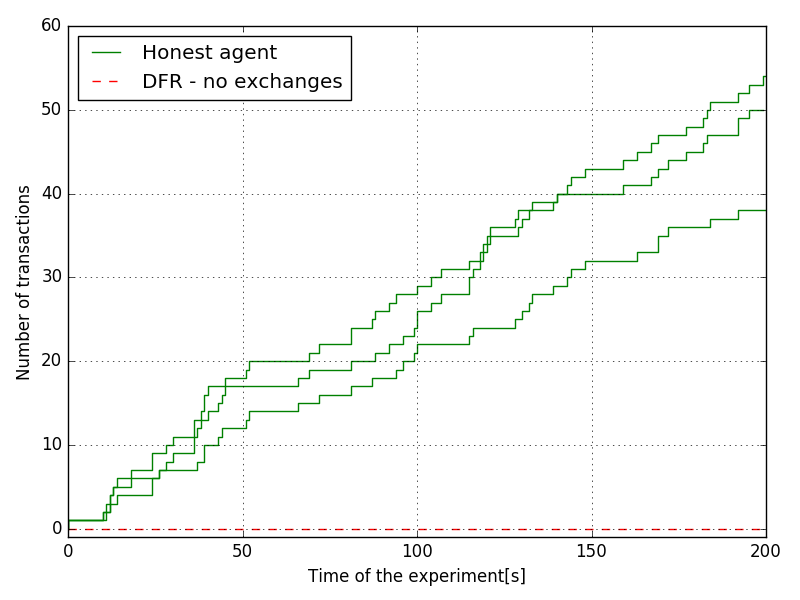
\includegraphics[width=.6\linewidth]{images/DFR_no_exchanges}
      \caption{Transactions over time of honest agents with dissemination free-rider that does not 
      perform any exchanges}
      \label{fig:DFR_no_exchanges}
    \end{subfigure}\\
    \begin{subfigure}{\textwidth}
      \centering
      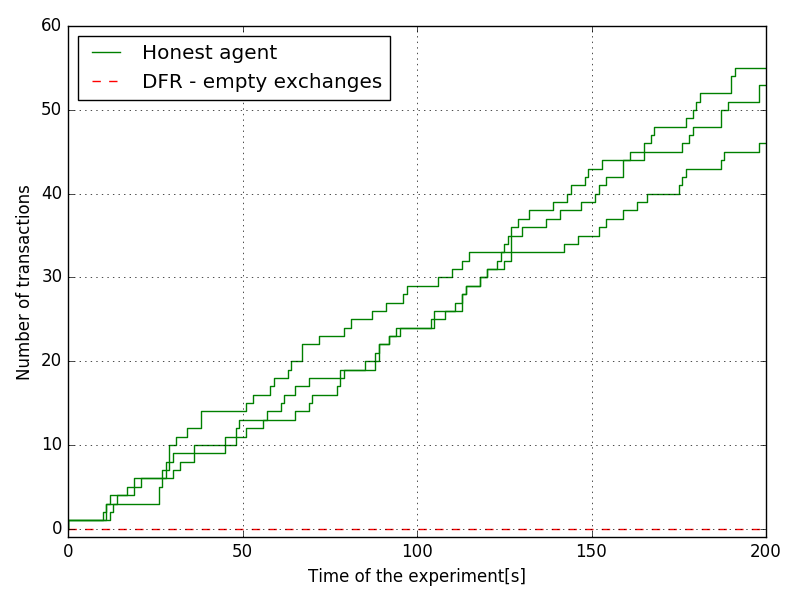
\includegraphics[width=.6\linewidth]{images/DFR_empty_exchanges}
      \caption{Transactions over time of honest agents with dissemination free-rider that creates 
      empty exchanges}
      \label{fig:DFR_empty_exchanges}
    \end{subfigure}\\
    \begin{subfigure}{\textwidth}
        \centering
        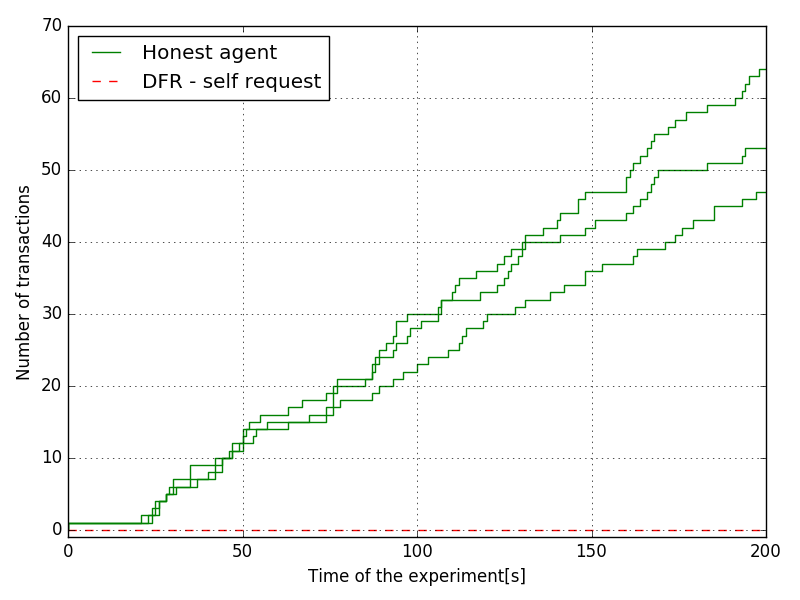
\includegraphics[width=.6\linewidth]{images/DFR_self_request}
        \caption{Transactions over time of honest agents with dissemination free-rider that only 
        exchanges own data}
        \label{fig:DFR_self_request}
      \end{subfigure}
\end{figure}

\subsection{Collaborating dissemination free-riders}

\begin{figure}[h!]
    \centering
    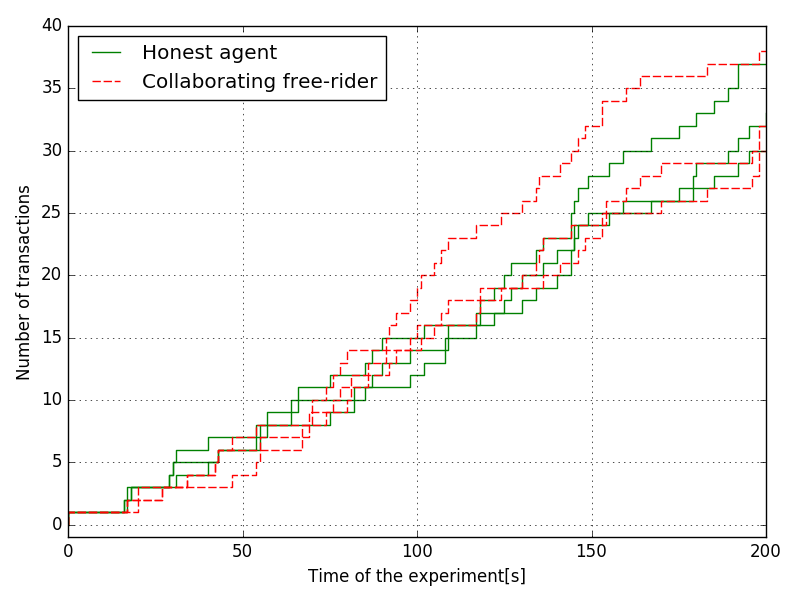
\includegraphics[width=0.7\textwidth]{images/50percent}
    \caption{Transaction history of three honest agents and three dissemination free-riders
    that are cooperating}
    \label{fig:50percent}
\end{figure}

\begin{figure}[h!]
    \centering
    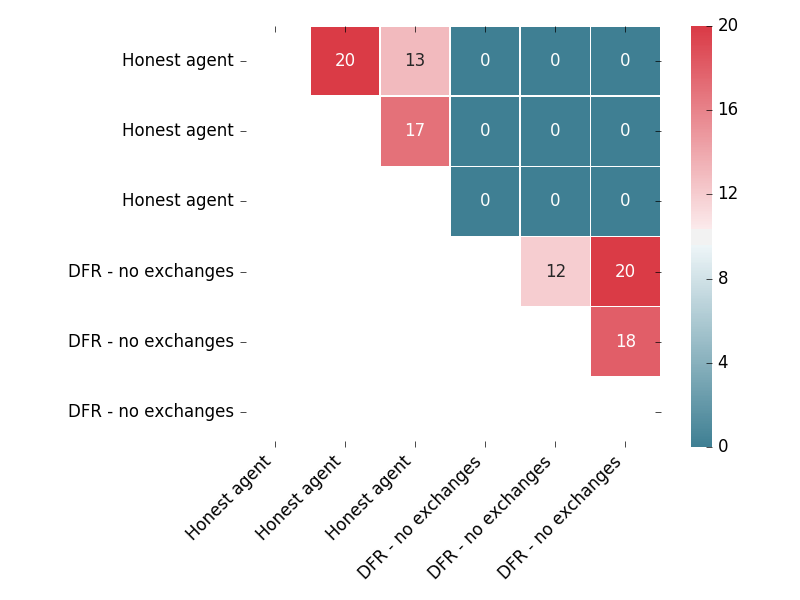
\includegraphics[width=0.7\textwidth]{images/50percent_interaction_matrix}
    \caption{Interaction matrix of three honest agents and three dissemination free-riders who are cooperating}
    \label{fig:50percent}
\end{figure}

\subsection{Malicious behavior}

\begin{figure}
    \begin{subfigure}{\textwidth}
      \centering
      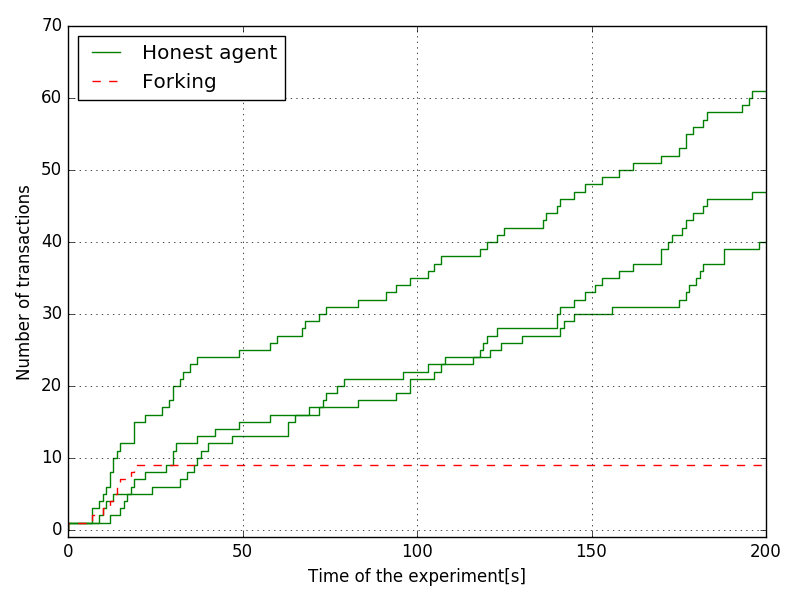
\includegraphics[width=.6\linewidth]{images/forking}
      \caption{Transaction history of three honest agents interacting with one strategic manipulator who performs a fork}
      \label{fig:forking}
    \end{subfigure}\\
    \begin{subfigure}{\textwidth}
      \centering
      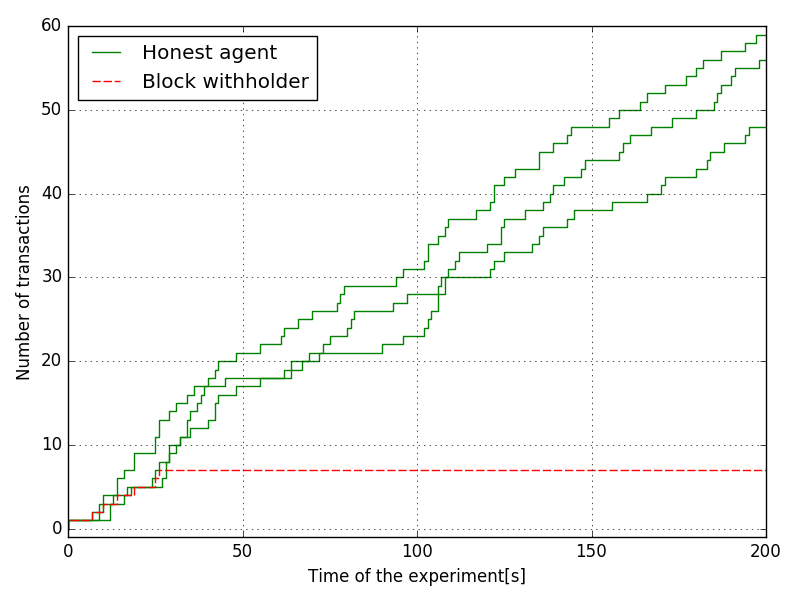
\includegraphics[width=.6\linewidth]{images/transaction_hiding}
      \caption{Transactions over time of three honest agents with one strategic manipulator who tries to hide a transaction}
      \label{fig:DFR_empty_exchanges}
    \end{subfigure}\\
\end{figure}

\subsection{Verification free-rider}

\begin{figure}
    \begin{subfigure}{\textwidth}
      \centering
      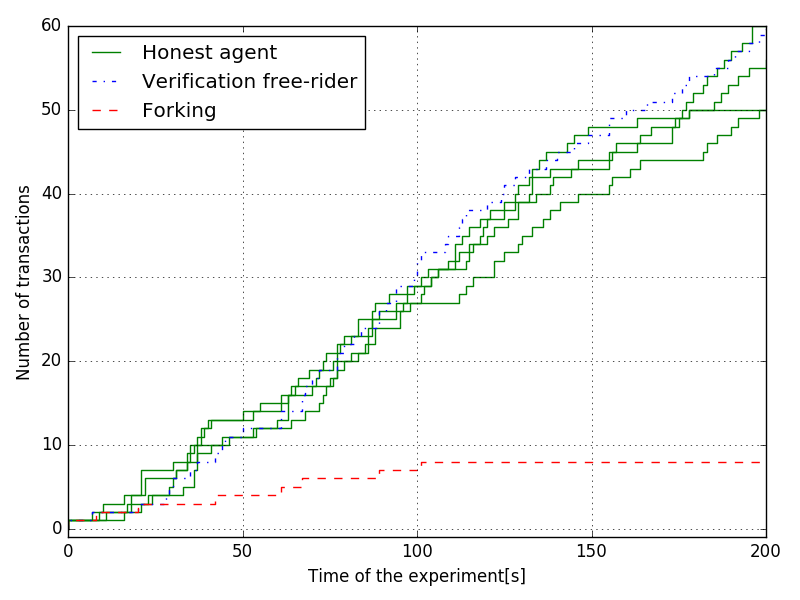
\includegraphics[width=.6\linewidth]{images/verification_doublespend_honest}
      \caption{Transaction history of three honest agents interacting with one strategic manipulator who performs a fork and a verification free-rider}
      \label{fig:verification_doublespend_honest}
    \end{subfigure}\\
    \begin{subfigure}{\textwidth}
      \centering
      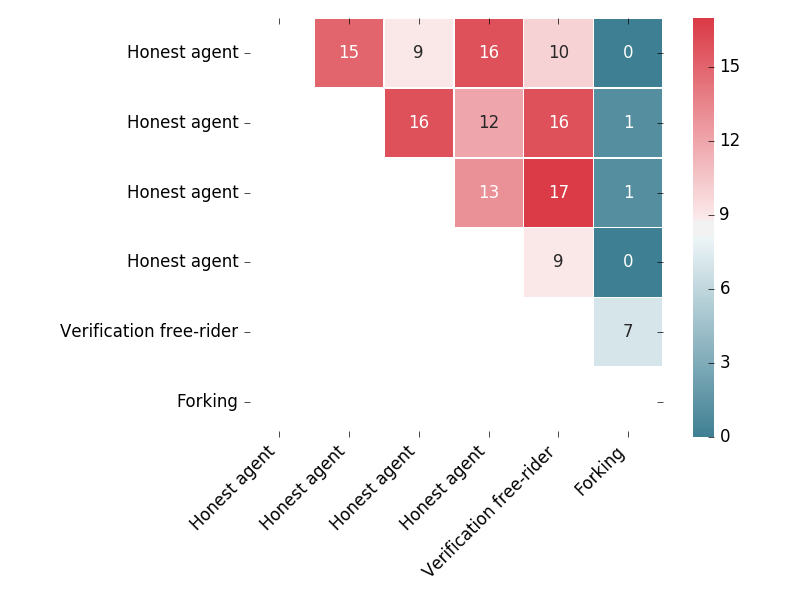
\includegraphics[width=.6\linewidth]{images/verification_doublespend_honest_matrix}
      \caption{Interaction matrix of three honest agents with one strategic manipulator who performs a fork and a verification free-rider}
      \label{fig:verification_doublespend_honest_matrix}
    \end{subfigure}\\
\end{figure}

\begin{figure}
    \begin{subfigure}{\textwidth}
      \centering
      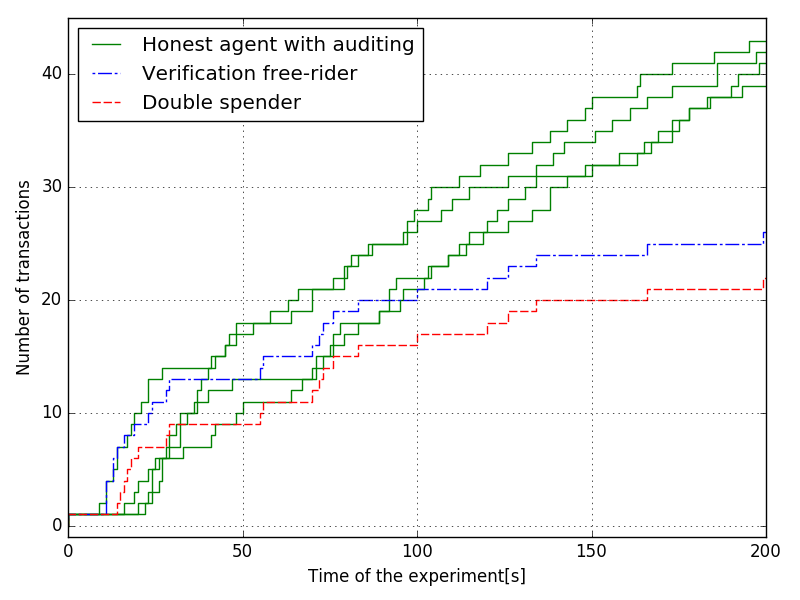
\includegraphics[width=.6\linewidth]{images/verification_doublespending}
      \caption{Transaction history of three honest agents with replay verification interacting with one strategic manipulator who performs a fork and a verification free-rider}
      \label{fig:verification_doublespending}
    \end{subfigure}\\
    \begin{subfigure}{\textwidth}
      \centering
      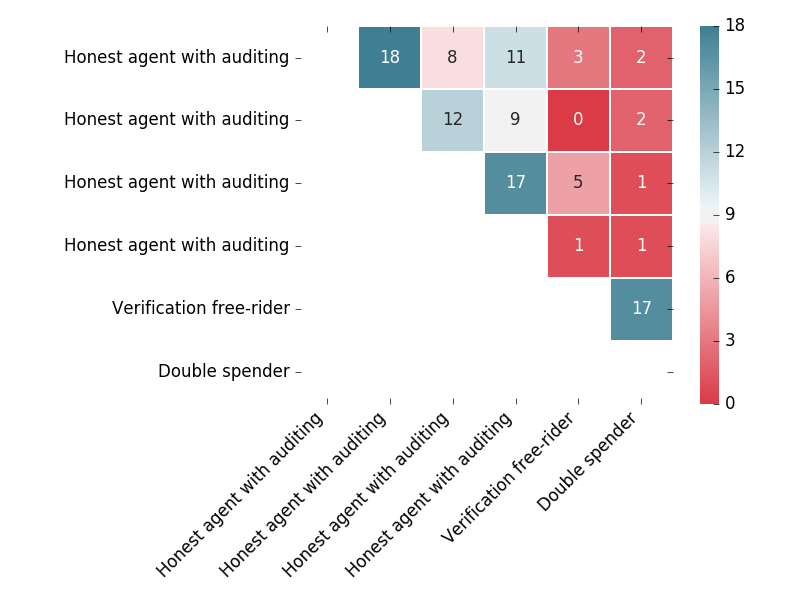
\includegraphics[width=.6\linewidth]{images/verification_doublespending_matrix}
      \caption{Interaction matrix of three honest agents with replay verification with one strategic manipulator who performs a fork and a verification free-rider}
      \label{fig:verification_doublespending_matrix}
    \end{subfigure}\\
\end{figure}

\section{}

\subsection{Sybil attack}

    \chapter{Discussion}
In this work we presented a strategy-proof mechanism for information dissemination. Applied to our 
distributed blockchain based trust system we are able to effectively defend against dissemination 
and verification free-riders. It creates an incentive for each agent on the network to help defend 
the network against any lazy or malicious behavior. It thereby is a major step towards a secure, 
distributed and scalable trust system.

* we defined a new blockchain system based on TrustChain which provides internal agent state 
transparency/gossip transparency
* we formally proof that the architecture provides a complete view of the internal state of the 
agent
* we defined a specific mechanism that makes use of the archiecture
* we experimentally proof that honest agents are able to eventually identify free-riders and malicious
agents

\section{Future research}

\subsection{Further developing this mechanism}
* incremental 
* research scalability properties for this mechanism
* locality by interacting with those that have similar information
* sybil attack resistance by checking that new agents paid their dues

\subsection{Next steps for the trust system}
* locality with ping
* 

    % \chapter{Mathematical framework}
Cooperation is, next to mutation and selection, an important factor in the evolution of organisms and communities. Cooperation is found in many species, but nowhere so prevalent as in humans, which is due to our superior abilities of communication and reasoning. It lead to the creation of modern society and our ever increasing welfare. Cooperation is driven by reciprocity, the exchange of good deeds or more colloquial: “I help you, you help me.” Reciprocity contrasts with selfishness, which opposes cooperation. Reciprocity is generally beneficial for both parties if they interact multiple times and have knowledge of their previous interactions (iterated prisoners’ dilemma). 


In the early days of human society, reciprocity was a key factor to create communities and settlements. Fast-forwarding to the modern time, communities are much larger with the most famous example being the internet. In such large communities, direct reciprocity often does not work anymore because there is an asymmetry in resources and abilities. “I help you, you help me.” only works if both parties can be of service to each other. In very large communities, the probability of interaction with the same party is very low. Also usually one party provides and the other party consumes the service, as seen with the sharing economy services like Airbnb or Uber. Then a concept known as indirect reciprocity comes into play which is directly tied to the concepts of trust and reputation. Colloquially, indirect reciprocity can be described as “I help you, someone helps me.” The intuition is then that nodes acquire a good reputation when acting altruistically and thus gain a higher chance of also receiving altruistic from the community. This requires an infrastructure to communicate the reputation of members of the community. The natural form of this communication in real-world communities is gossip. More and more online communities are using such a reputation system to improve the reciprocity and reliability of their service. They use central databases to keep track of the reputations of all users. This has advantages: the central database is available, searchable and complete. However, the disadvantages are severe: each service and community on the internet uses it’s own reputation system with different rules, scales and information which cannot be accessed by it’s users. This means the company is owner of the reputation of all its users and not the users themselves. A driver on Uber cannot take her reputation to Lyft but has to start new. Also, users cannot combine all their different reputations to build up a digital profile of themselves as proof of their trustworthiness to new communities they join. What we are missing is a universal reputation database to create trust between unrelated parties in the very large online community. The reputation database should be owned by and accessible to everyone, scale horizontally and be tamper-proof.


We envision a decentralized, multi-chain based reputation system with linear scalability. \textbf{Interactions} between users (nodes) are recorded on their personal blockchain according to the TrustChain protocol~\cite{trustchain-protocol}. Based on the history of a node’s interactions it has a reputation in the system and other nodes trust it to a certain extent, given by the expected value of cooperation in future interactions. Encounters, reputation and trust exist in a certain context. Contexts influence each other. 

Reputation systems in general and distributed reputation systems in particular pose some challenges to the designer:

\begin{itemize}
    \item Reputation systems can be subject to the sybil-attack: an attacker creates a large number of fake nodes which endorse the attacker with high reputation which the attacker can subsequently take advantage of. 
    \item A distributed network is not fully connected: not all nodes are online at all times and information could be missing
    \item In a distributed system we are reliant on nodes sending correct information but they can reject connections or send wrong information
\end{itemize}

In previous work we have shown that we can record encounters in a multi-chain system, calculate subjective reputation of other nodes to prevent freeriding and make the reputation ranking sybil-resilient. However the calculation of reputation is local and subjective. This is problematic: if an agent acts altruistically, she can only benefit if nodes are aware that she did. In this work we focus on a way to distribute the personal views of reputation of nodes on the network to work towards consensus on the reputation of nodes.


For simplicity, we assume a single context for the following definition of the key concepts which are the basis for this reputation system.
We consider a distributed network of $n$ entities. We borrow the definitions for the interaction model from~\cite{trustchain}.

\paragraph{Definition 1} (\textit{Ordered interaction model}). An ordered interaction model $M=\langle P,I,a,w\rangle$ consists of two sets and two functions.
\begin{itemize}
    \item $P$, a finite set of agents
    \item $I$, a finite set of interactions
    \item $a : I \rightarrow P \times P$, a function mapping each interaction to the agents involved in it.
    \item $w : I \times P \rightarrow \mathbb{R}_{\leq0}$, a function which describes the contribution of an agent in an interaction
\end{itemize}

Evidence of interactions are recorded in blocks on the personal hashchains of agents. In practice, each node is aware of a subset of the interactions and nodes in the network.

\paragraph{Definition 2} (\textit{Subjective interaction history}). A subjective interaction history $H_p = \langle P_p, I_p, a_p, w_p \rangle$ defines the knowledge of an agent $p$.
\begin{itemize}
    \item $P_p$, a finite set of agents known to $p$
    \item $I_p$, a finite set of interactions known to $p$
    \item $a_p : I_p \rightarrow P_p \times P_p$, a function mapping each interaction to the agents involved in it
    \item $w_p : I_p \times P_p \rightarrow \mathbb{R}_{\leq0}$, a function which describes the contribution of an agent in an interaction
\end{itemize}

\paragraph{Definition 3} (\textit{Interaction evidence}). Evidence of interactions is stored in form of transaction blocks on personal blockchains. One block $b_{p,i} = \langle H(b_{p,i-1}),{seq}_p, {txid}, {pk}_q, w, {sig}_p \rangle$ correspondes to one interaction $i \in I$. $B_p,p$ is then the set of blocks that are the evidence of the personal interactions $I_p,p = \{ i \in I : p \in a(i) \}$ of node $p$. An agent $p$ has a \textbf{subjective interaction evidence} $B_p$ which is the set of blocks corresponding to all interaction $I_p$ known to agent $p$.

\paragraph{Definition 4} (\textit{Reputation mechanism}). A reputation mechanism is function that maps from a subjective interaction evidence $B_p$ to a set of reputation values, $F: B_p \rightarrow \mathbb{R}^{\lvert P_p \rvert}$, where $F_q(B_p)$ is the reputation of agent $q$ as seen by node $p$.

\paragraph{Definition 5} (\textit{Private information set}). An agent $p$ has a private information set $\mathbb{I_p} = \langle B_p, F(B_p), A_p \rangle$. 
\begin{itemize}
    \item $B_p = B_p,p \cup B_p,-p$ the set of blocks known to agent $p$, defined as the union of $B_p,p$, the blocks of interactions which involved agent $p$, and $B_p,-p$, the blocks of those interactions which did not involve agent $p$
    \item $F(B_i)$ is a reputation ranking of all nodes known to agent $p$, given the evidence $B_p$, calculated using a reputation mechanism $F$
    \item $A_p = \{\langle pk_q, B_{p+q}^{(t)},F_q(B_{p+q}^{(t)})\rangle \}$ is the set of auditions (defined later), that have engaged in pairwise auditing with agent $p$
\end{itemize}

\paragraph{Definition 6} (\textit{Pairwise audition}). A pairwise audition is an exchange of private information between agents $p$ and $q$ such that after audition both agents have the same subjective interaction evidence $B_{p}^{(t+1)} = B_{q}^{(t+1)}= \{B_p,p^{(t)}, B_p,-p^{(t)}, B_q,q^{(t)}, B_q,-q^{(t)} \}$, both agents add their results to their set of auditions, $A_p^{(t+1)} = A_p^{(t)} \cup \{\langle pk_q, B_{p}^{(t+1)},F_q(B_{p}^{(t+1)})\rangle\}$

After a pairwise audition agent $p$ knows about the correctness of node $q$'s chain and disseminate 

    %% Use letters for the chapter numbers of the appendices.
    \appendix
    
    %\input{appendix-a}
    
    \bibliography{report}
    
    \end{document}
    
    
